
% This template has been edited from the IEEE template available at:
% https://www.ieee.org/conferences/publishing/templates.html
%
% For further help, you may wish to see:#
% https://www.overleaf.com/learn/latex/tables
% https://www.overleaf.com/learn/latex/Inserting_Images
% https://www.overleaf.com/blog/532-creating-and-managing-bibliographies-with-bibtex-on-overleaf

\documentclass[conference]{IEEEtran}
%\IEEEoverridecommandlockouts
% The preceding line is only needed to identify funding in the first footnote. If that is unneeded, please comment it out.
\usepackage[a4paper, total={6in, 8in}, margin=0.75in]{geometry}
\usepackage{cite}
\usepackage{amsmath,amssymb,amsfonts}
%\usepackage{algorithmic}
\usepackage{algorithm} 
\usepackage{algpseudocode} 
\usepackage{graphicx}
\usepackage{textcomp}
\usepackage{xcolor}
\def\BibTeX{{\rm B\kern-.05em{\sc i\kern-.025em b}\kern-.08em
    T\kern-.1667em\lower.7ex\hbox{E}\kern-.125em}}
\begin{document}

\title{Report Title: Be Descriptive}

\author{
    \IEEEauthorblockN{Student Number}
    \and
    \IEEEauthorblockN{Student Number}
}

\maketitle

\begin{abstract}
It is normal to write the abstract last.  First, try to concisely state the problem/question/challenge under investigation.  Second, state what you found out.  The abstract should help a reader decide if they are interested in reading the whole paper.  
\end{abstract}


\section{Introduction}
Use the introduction to explain your project (problem/question/challenge) to the reader.  To do this well, you will need to provide some background context.  It can be useful to imagine you are writing for someone who would be able to understand your work, but who is not familiar with it.  You should assume the examiner of this report has \textbf{not} seen your project before.   

For example, you may need to explain how a sensor works, including the advantages and disadvantages, in order for your reader to properly understand the \emph{value} of your investigation.  You want your reader to agree that this is an interesting project, as well as for your reader to understand \emph{why}. 

You are encouraged to use specialist language and concepts covered in the unit to explain the background context of your project.  Where relevant, you are encouraged to reference external sources of information, such as technical datasheets, online articles\cite{picard2001toward}\cite{beck2010towards}, or academic literature.  Try to write your report both to explain it well and to demonstrate what you have learnt.

\subsection{Hypothesis Statement}

Because formulating a hypothesis is central to this assessment, it is recommended you write your hypothesis into a clear subsection (this subsection) as specified in this report template.  Because you have introduced your work well above (providing key background context and specialist knowledge) you can be quite literal here with your hypothesis.  For example: 

Because the VL1680X has been identified as an active sensor with ... limitations, we hypothesise that:
\begin{quote}
    by applying ... filtering to the sensor, we predict a measurable improvement of the sensor under ... conditions.  
\end{quote}

We investigate this hypothesis through a structured experiment on the Pololu 3Pi+ mobile robot, comparing the performance of the sensor with and without our technique.  

\section{Implementation}
% 2.
% 在这一节中,你应该描述你的实现的具体细节,以便你的读者可以重新创建你的工作。  
% 如果你使用了一个已经被广泛理解的算法或技术,你可以只参考一个外部来源而不详细解释,除非解释算法/技术为读者提供了关于你的项目的重要信息。 
% 你可能希望在这里介绍技术信息,以支持对特定组件的理解(例如,一个传感器或执行器的响应图,或者如果你在实验前有一个早期的可行性研究)。
% 如果你要将你的机器人系统与自己进行比较,那么你可能需要记录你的 "基础"解决方案和你的 "改进版"解决方案。  
In this paper we have measured the performance of the PID controller with the Pololu 3pi+ 32U4 robot. We implemented the robot's wheel motor control, wheel speed measurement and PID control of the wheel speed in software.
% 本文中,对PID控制器的性能是在Pololu 3pi+ 32U4 Robot身上展开的。我们用软件实现了机器人的轮子电机控制,速度追踪,以及对轮子速度的PID控制。

% 插入系统框图
\begin{figure}[htbp]
\centerline{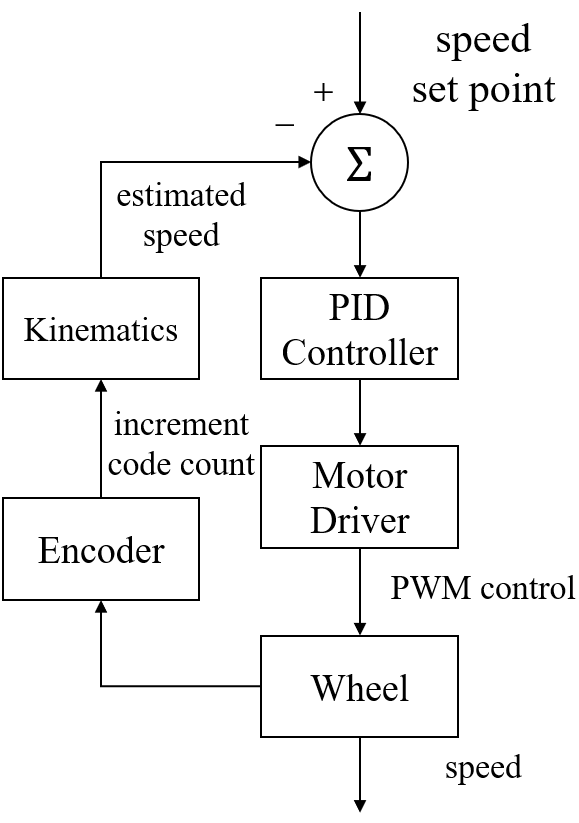
\includegraphics[width=0.6\linewidth]{Report/Pic/ImplementFLowChart.png}}
\caption{System Components.}
\label{fig1}
\end{figure}

% 系统主要有5个组成部分:PID控制器,Motor Driver,Wheel,Encoder, Kinematics
System has 4 main components: PID controller, Motor Driver, Wheel, Encoder, Kinematics. They are structured as shown in Fig. \ref{fig1}. 
\begin{itemize}
    \item\textbf{PID Controller: } We use a basic PID controller in our system to minimise the number of irrelevant variables. We do not want popular improvements to the PID to become variables in the system, such as integral limitation. The PID controller we use can be described as below:
    
    
        \begin{equation}\label{PID_1}
            e(t) = r(t) - y(t)      
        \end{equation}
        $r(t)$: set point value, or say the aim of the system\\
        $y(t)$: system output \\
        $e(t)$: error
        \begin{equation}\label{PID_2}
            u(t)=K_{p}*e(t)+K_{i} * \sum_{i=1}^{k}  (e(t_{i})\Delta t)+K_{d} * \frac{de(t)}{dt}
        \end{equation}
        $u(t)$:PID controller output
        \par
    \item\textbf{Wheel and Motor Driver: }For Pololu 3pi+ 32U4 robot, user could control the motor speed by controlling motor PWM duty cycle ratio. Motor takes 0$\sim$255(integer) as input and output 0$\sim$5V power to the motor.
    %插入电机速度与输入的特性图 %
    % 也就意味着速度计算有一些误差(难以测得一圈的编码数),但速度误差对本文中的实验没有影响。
    \item\textbf{Encoder: }Each wheel shaft has an encoder that can be used to measure the movement of the wheel. Encoder counts between 358$\sim$359 for a 360° wheel spin. It also means that there is some error in the velocity calculations (it is difficult to measure the exact code count of one lap), but the velocity error has no effect on the experiments in this paper.
    % 用编码器值的变化与轮子的周长计算轮子的运动,藉此计算机器人kinematics。在本文中只需计算运动学中的轮子速度部分。
    \item\textbf{Kinematics: }The motion of the wheel is calculated using the variation of the encoder value with the circumference of the wheel in order to calculate the robot kinematics. in this paper only the wheel speed part of the kinematics is needed.

\end{itemize}

\begin{figure}[htbp]
\centerline{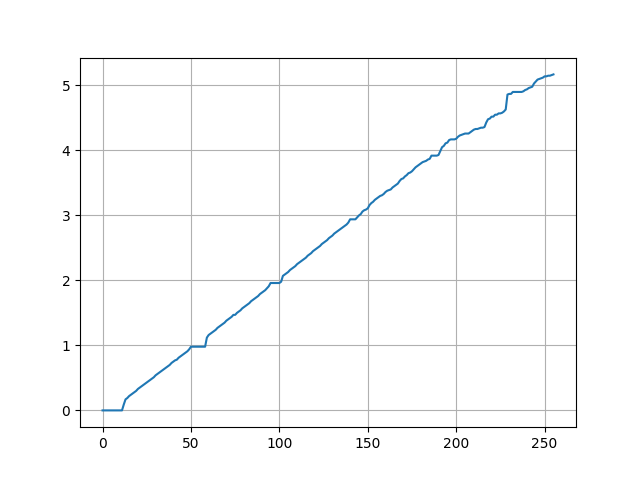
\includegraphics[width = 300]{Report/Pic/WheelResponse.png}}
\caption{System Components.}
\label{fig1}
\end{figure}


\begin{algorithm}
	\caption{Pseudo Codes}\label{pseudo:ppo}
	\begin{algorithmic}[1]
		\For {$iteration=1,2,\ldots$}
			\For {$actor=1,2,\ldots,N$}
				\State Run policy $\pi_{\theta_{old}}$ in environment for $T$ time steps
				\State Compute advantage estimates $\hat{A}_{1},\ldots,\hat{A}_{T}$
			\EndFor
			\State Optimize surrogate $L$ wrt. $\theta$, with $K$ epochs and mini-batch size $M\leq NT$
			\State $\theta_{old}\leftarrow\theta$
		\EndFor
	\end{algorithmic} 
\end{algorithm}

\section{Experiment Methodology}
% 3.
% 在这一节中,记录你是如何组织(设计)你的实验的,从而使其他人可以很容易地重新创造你的工作。  
% 你也希望你的读者同意你仔细考虑了你的实验,这样我们就可以相信你的结果是有意义的,而且是可信的(没有错误)。 
% 你在这一节中使用哪些小节(如果有的话),主要取决于你的项目和你选择的展示方式。  以下是一些建议,以帮助你的工作清晰化。
In this section, document how you structured (designed) your experiment such that someone else could easily recreate your work.  You also want your reader to agree that you carefully considered your experiment so that we could trust your results to be both \emph{insightful} (mean something) and \emph{credible} (not subject to error).  Which subsections (if any) that you use in this section will largely depend on your project and how you choose to present it.  The following are suggestions to aid the clarity of your work.

\subsection{Overview of Method}
% 3.A
% 向读者描述你的实验的一般结构和程序。你应该提供一个有点像蛋糕食谱的规格。 
% 例如:你的实验持续多长时间? 你使用多少次重复试验?有多少种备用方案?
Describe to the reader the general structure and procedure of your experiment. You should provide a specification a bit like a cake recipe.  For example: how long does your experiment last?  how many repeated trials do you use?  how many alternate scenarios are there?

\subsection{Discussion of Variables}
% 3.B
% 你应该概述一下你的实验中的关键变量。这将有助于你的读者以后相信你的结果是可信的,而不会读不懂。
You should outline the key variables within your experiment. This will help your reader to later believe your results are credible and not confused.
\begin{itemize}
    % 变量表
    % 受控变量:这些是你的实验(任务、硬件、软件、环境)的部分,这些部分可能会有变化,但你通过仔细设计实验来控制它们。例如,电池寿命不同,所以你将使用新电池。
    \item \textbf{Controlled Variables}: These are the parts of your experiment (task, hardware, software, environment) which \emph{could} vary, but which you have controlled by careful design of your experiment.  For example, battery life varies, so you will use new batteries.
    % 自变量:这是你要改变的实验部分,以便你希望观察到性能的可测量的改变。  请注意,我们曾经只想要一个自变量--有时我们以此为目标,但承认其他部分会发生变化,我们需要对我们的系统和/或结果进行仔细分析。
    \item \textbf{Independent Variable}: This is the part of your experiment which you are changing so that you hope to observe a measurable alteration in performance.  Note that, we ever only want one independent variable - sometimes we aim for this, but concede other parts will change, and we need to make careful analysis of our system and/or results.
    % 因变量:这些是你的实验的一部分,你希望在其中观察到一个可测量的变化。  你将设计或选择适当的参数来测量和分析这个可依赖的变量。  例如,我们可以有一个系统的因变量,但使用平均值、模式和中位数的指标来分析它。
    \item \textbf{Dependent Variable(s)}: These are the part(s) of your experiment in which you hope to observe a measurable change.  You will design or select appropriate \emph{metrics} to measure and analyse this dependable variable.  For example, we can have one dependent variable of the system, but use metrics of mean, mode and median to analyse it.
\end{itemize}

\subsection{Discussion of Metric(s)}
% 3.C 讨论参数
% 在这一部分,你应该讨论你选择指标的理由(为什么)--例如,这些指标如何帮助我们解释你的结果?  你的衡量标准需要在整个实验中得到一致的应用,以便提供性能的比较。  
% 你应该讨论你的衡量标准的优点和缺点。  通常,我们需要一个以上的指标来弥补另一个指标中被混淆或隐藏的信息。  通过使用一个以上的指标,我们可以更接近于你的实验结果的真相。  
 In this section you should discuss the rationale (why) you have selected your metric(s) - e.g. how do these metrics help us to interpret your results?  Your metric(s) will need to be applied consistently throughout your experiment for them to provide a comparison of performance.  
 
 You should discuss the advantages and disadvantages of your metric(s).  Often, we need more than one metric to compensate for the information which is confused or hidden in another metric.  By using more than one metric, we can get closer to the truth of the outcome of your experiment.  

\section{Results}
% 4.
% 在这一部分中,你应该介绍你的结果。 
% 一般来说,最好是既要有 "定量 "的结果(如数据),又要有 "定性 "的结果(如有代表性的书面观察或图表)。  

% 你应该在有助于清晰的地方使用分节。 
% 例如,先介绍 "基础"系统的结果,然后介绍 "改进后"系统的结果,最后介绍同时考虑 "基线 "和 "改进 "系统的结果,这可能是有用的。  
% 然而,这将完全取决于你的项目和你如何设计你的实验。

% 在介绍结果时,应力求在介绍中清楚地传达一种见解。
% 例如,一张包含所有单个数据的大表需要读者做大量的工作来找出重要的内容。 
% 与此相反,一个适当展示平均数和标准差的表格已经为读者总结了结果(而且会更有用)。  
% 同样,在可能的情况下,将数据合并到图表中,以便进行直接比较--在可能的情况下,包括误差条。  
In this section you should present your results.  In general, it is best to aim for both \emph{quantitative} results (e.g., data) and \emph{qualitative} results (e.g., a written observation or graphic which is representative).  

You should use subsections where they aid in clarity.  For instance, it may be useful to present results for a ``baseline" system, then a results for an ``improved" system, and then finally results which consider both ``baseline" and ``improved" systems together.  However, this will depend entirely on your project and how you have designed your experiment.

When presenting results, aim for a presentation which clearly communicates an insight. For example, a large table of all the individual data requires the reader to do a lot of work to find out what is important.  In contrast, a table which appropriately presents the mean and standard deviation has summarised the results for the reader (and would be more useful).  Similarly, aim to combine data onto a chart when possible so that a direct comparison can be made - and when possible, include error bars.  


% 记住标明所有的轴线,给所有的图表、数字和表格加上标题,并在报告文本中引用这些内容(例如,见图ref{fig1})
% --永远不要要求读者必须自己得出结论或理解,解释他们正在看什么。  
% 记住要尝试对你的结果中的任何异常情况做出解释。  
Remember to label all axis, caption all graphs, figures and tables, and to reference these elements in the report text (e.g. see figure \ref{fig1}) - never require a reader to have to come to their own conclusion or understanding, explain what they are looking at.  Remember to attempt to give an explanation for any anomalies in your results.  


\section{Discussion and Conclusion}
% 5.
% 通过重新陈述你的假设来开始你的讨论和结论。  你可以在这里复制和粘贴你的假设。  
Begin your discussion and conclusion by re-stating your hypothesis.  You can literally copy-and-paste your hypothesis here.  
% 下面两行是示例:
Because the VL1680X has been identified as an active sensor with ... limitations, we hypothesised that:
\begin{quote}
    by applying ... filtering to the sensor, we predict a measurable improvement of the sensor under ... conditions.  
\end{quote}
% 对你的结果进行讨论--这是否支持或反驳了你的假说。 
% 结果可能是混合的(支持和反驳),你应该在这里讨论。
% 在你的讨论中,将此作为另一个展示/证明你的理解的机会。尽量避免陈述显而易见的事情
% --相反,用分析/评价/综合来表明你了解你是如何和为什么看到这样的结果的。 
% 你的发现有什么意义?  
Make a discussion of what your results showed - whether this supported or refuted your hypothesis.  It may be that the results were mixed (supporting and refuting) and you should discuss that here. In your discussion, use this as another opportunity to demonstrate/evidence your understanding. Try to avoid stating the obvious - instead, use analysis/evaluation/synthesis to show that you understand \emph{how} and \emph{why} you saw the results you did.  What are the implications of your findings?  
% 这也是评估你的实验和项目整体的一个好机会。  
% 你可能希望进一步讨论研究的局限性(例如,控制/自变量的难度,或你在项目中面临的任何问题)。 
% 你可能希望对未来的工作提出建议--但要确保这是从你所获得的理解中获得的明确进展,而不是胡乱猜测。
This is also a good opportunity to evaluate your experiment and project as a whole.  You may wish to further discuss the limitations of the study (e.g. the difficulty of controlled/dependent variables, or any problems you faced in your project).  You may wish to make a recommendation for future work - but ensure that this is a clear advancement from the understanding you have gained and not wild speculation.


\bibliographystyle{ieeetr} 
\bibliography{biblio}


\end{document}
